%%
%% This is file `sample-xelatex.tex',
%% generated with the docstrip utility.
%%
%% The original source files were:
%%
%% samples.dtx  (with options: `sigconf')
%% 
%% IMPORTANT NOTICE:
%% 
%% For the copyright see the source file.
%% 
%% Any modified versions of this file must be renamed
%% with new filenames distinct from sample-xelatex.tex.
%% 
%% For distribution of the original source see the terms
%% for copying and modification in the file samples.dtx.
%% 
%% This generated file may be distributed as long as the
%% original source files, as listed above, are part of the
%% same distribution. (The sources need not necessarily be
%% in the same archive or directory.)
%%

\documentclass[sigconf, nonacm]{acmart}

\usepackage{mwe}
\usepackage[colorinlistoftodos,prependcaption,textsize=tiny]{todonotes}


%%
%% \BibTeX command to typeset BibTeX logo in the docs
\AtBeginDocument{%
  \providecommand\BibTeX{{%
    \normalfont B\kern-0.5em{\scshape i\kern-0.25em b}\kern-0.8em\TeX}}}

\begin{document}

%%
%% The "title" command has an optional parameter,
%% allowing the author to define a "short title" to be used in page headers.
\title{Express Data Queueing}

%%
%% The "author" command and its associated commands are used to define
%% the authors and their affiliations.
%% Of note is the shared affiliation of the first two authors, and the
%% "authornote" and "authornotemark" commands
%% used to denote shared contribution to the research.
\author{Freysteinn Alfreðsson}
\email{freysteinn.alfredsson@kau.se}
\orcid{0000-0003-1516-9370}
\affiliation{%
  \institution{Department of Computer Science}
  \city{Karlstad}
  \country{Sweden}
}
\author{Per Hurtig}
\email{per.hurtig@kau.se}
\affiliation{%
  \institution{Department of Computer Science}
  \city{Karlstad}
  \country{Sweden}
}
%%\orcid{0000-0003-1516-9370}
\author{Anna Brunstrom}
\email{anna.brunstrom@kau.se}
\affiliation{%
  \institution{Department of Computer Science}
  \city{Karlstad}
  \country{Sweden}
}

\author{Toke Høiland-Jørgensen}
\email{toke@redhat.com}
\affiliation{%
  \institution{Red hat}
  \country{Denmark}
}

\author{Jesper Dangaard Brouer}
\email{brouer@redhat.com}
\affiliation{%
  \institution{Red hat}
  \country{Denmark}
}

%%
%% By default, the full list of authors will be used in the page
%% headers. Often, this list is too long, and will overlap
%% other information printed in the page headers. This command allows
%% the author to define a more concise list
%% of authors' names for this purpose.
\renewcommand{\shortauthors}{Alfreðsson, et al.}

\begin{abstract}
\end{abstract}

%%
%% Keywords. The author(s) should pick words that accurately describe
%% the work being presented. Separate the keywords with commas.
\keywords{XDP, eBPF, BPF, Queueing, Linux, Scheduling}

%%
%% This command processes the author and affiliation and title
%% information and builds the first part of the formatted document.
\maketitle

\section{Introduction}

The Linux kernel is a widely used platform in devices that range from IoT
devices, cellphones, home and enterprise routers to servers and cloud offerings.
One of the revolutionary technologies of the Linux kernel is the BPF framework,
which has changed the way we extend the kernel. This framework is an in-kernel
runtime environment that allows domain-specific code to execute within the
kernel safely using predefined hooks. One such hook is the Linux eXpress Data
Path\cite{hoiland2018express}, or XDP, which has found numerous uses in the
industry, such as DoS attack mitigation, load-balancers, and intrusion
prevention systems.

XDP provides a high-performance programmable network data path and allows
programmers to process packets early out of the driver. While XDP excels in
forwarding packets, it currently has no mechanism for queueing or reordering
packets and cannot implement traffic scheduling policies.

Packet scheduling is a common task on network equipment, which it uses to
prioritize different traffic between hosts. On smartphones, the packet scheduler
might want to prioritize video streaming over application updates. A cloud
provider might wish to schedule fairness between customers or even prioritize
some customers over others. With the growing number of devices and their diverse
network requirements, there is a need for increased flexibility in the rapid
deployment and interaction with schedulers.

This paper presents our work on adding programmable packet scheduling to XDP,
which we also provide as a Qdisc. We have designed a programmable packet
scheduling framework in BPF using recently proposed schemes for programmable
queues. This extension allows programmers to define their packet schedulers
using BPF while benefiting from the XDP fast data path.


\begin{itemize}
\item Explain the structure of this technical report.
\end{itemize}

\section{Packet Scheduling, Traffic Shaping, and Queue Management}

The main function of the packet scheduler is to arrange or rearrange packets
in order to meet some specific criteria. However, they can also be used to shape
traffic.

\todo[inline]{Frey: This text should not sound like it is explaining packet scheduling from scratch. We assume that the audience have the main overview of what a packet scheduler is.}

\begin{itemize}
  \item Explain the basic concepts of packet schedulers.
  \item Explain the difference between schedulers and queues.
  \item Explain the difference between a work-conserving and non-work conserving scheduling.
  \item Use a short round-robin scheduling example.
\end{itemize}

\section{Linux Kernel Networking Subsystem}

\begin{itemize}
  \item Explain on a high level the Linux Kernel Networking stack using a diagram.
\end{itemize}

\subsection{The Linux Kernel Packet Queueing Discipline (Qdisc)}

\begin{itemize}
  \item Explain where in the network pipe the Qdiscs are located.
  \item Explain, without going into too much detail, what the Qdisc system is capable of.
        \begin{itemize}
          \item Shaping: Shaping delay packets to meet a desired rate.
          \item Scheduling: Schedulers arrange and/or rearrange packets for output.
          \item Classifying: Classifiers sort or separate traffic into queues.
          \item Policing: Policiers measure and limit traffic in a particular queue.
          \item Dropping: Dropping discards an entire packet, flow or classification.
          \item Marking: Marking is a mechanism by which the packet is altered.
        \end{itemize}
  \item Explain what type of primitives the Qdiscs system supplies:
        \begin{itemize}
          \item Classfull Qdiscs.
          \item Classless Qdiscs.
          \item Filters.
        \end{itemize}
\end{itemize}


\section{Packet Schedulers in Practice}

\todo[inline]{Frey: This section needs a new name. The idea with this section is to explain why we care about this work and what the requirements are.}

\begin{itemize}
  \item Explain what is not possible using today's packet schedulers.
  \item Explain why you would like to be able to schedule traffic
\end{itemize}


\section{Programmable Packet Schedulers}

\todo[inline]{Frey: Maybe this section could be combined with the above section if we find a better name for them.}

\begin{itemize}
  \item Explain how programmable packet schedulers differ from traditional schedulers.
  \item Explain what we want from a programmable packet scheduler.
        \begin{itemize}
          \item Can handle work and non-work conserving scheduling.
          \item Can combine data structures to form a hierarchy for more advanced algorithms.
        \end{itemize}
\end{itemize}

\todo[inline]{Frey: In the original draft I had a special section called algorithm for each of the data structures below. I decided to remove it for now because I think it is intertwined with the data structure.}


\subsection{PIFO and SP-PIFO}

\begin{itemize}
  \item Explain what PIFO\cite{Sivaraman2016} is.
  \item Explain how PIFO does not allow scheduling at dequeue, but can form hierarchies to create more complex logic.
  \item Explain that SP-PIFO\cite{Alcoz2020} approximates the behavior of a PIFO using Strict-Priority queues.
  \item Explain that does not support non-work conserving scheduling.
\end{itemize}


\subsubsection{Data Structure}

\begin{itemize}
  \item Explain how the PIFO is an array of queues.
  \item Explain how the PIFO tends to not scale with large sizes. Mainly in hardware based scheduling.
  \item Explain how the SP-PIFO is a small PIFO that approximates larger PIFO.
\end{itemize}


\subsection{Eiffel}

\begin{itemize}
  \item Explain how Eiffel\cite{Saeed2019} data structure is designed for software based scheduling and that it is optimized using find-first-set instructions.
  \item Explain that it can change the order of the packets on dequeue, unlike PIFO.
\end{itemize}


\subsubsection{Data Structure}

\begin{itemize}
  \item Explain that it uses a bitmap to keep track of available slots for optimization with FFS commands.
  \item Explain that it uses two alternating data structures to allow incremental inserts while not needing to scale the bitmaps dynamically.
\end{itemize}


\subsection{Calendar-queues}

\begin{itemize}
  \item Explain that it supports both work and non-work conserving scheduling.
\end{itemize}


\subsubsection{Data Structure}

\begin{itemize}
  \item Explain that it uses a circular buffer with a hand like an analog clock. The slots represent when the scheduler will dequeue in the future. While the hand points to the packets that are dequeing.
\end{itemize}


\section{The extended Berkeley Packet Filter (eBPF)}

The eBPF framework is an in-kernel runtime environment that allows specialized
programs to execute in the kernel safely. These programs attach themselves to
hooks provided by the different subsystems of the kernel. These hooks limit what
the programs can do and define what type of eBPF programs can exist. These types
of programs vary but predominantly, they are related to networking, tracing, and
security. At its core, eBPF is an instruction set. However, as a framework, it
provides a key-value store that enables inter-process communication called eBPF
maps, in-kernel helper functions, and toolchains to create and manage eBPF
programs from user-space.

\todo[inline]{Frey: Because we all know what eBPF is, I am going to collapse these eBPF sections and make it shorter and simpler.}

\begin{itemize}
  \item Explain h
  \item Explain eBPF maps and their scope.
  \item Explain what hooks are and that eBPF allows helper functions.
  \item Explain how eBPF programs are loaded using the bpf system call.
\end{itemize}


\subsection{Instruction-set}

\todo[inline]{Frey: I think I will remove this section either completely, or at least remove the extra details.}

The eBPF instruction set is 64-bit and consists of eleven registers listed in
table ~\ref{table:eBPF_registers}. It contains a little over a hundred
instructions. However, the current format defines the opcode as the first octet
of the instruction. Therefore, in the current design, it could only support 256
instructions. The currently available instructions are limited to Arithmetic
Logic Unit (ALU) instructions, byte-swap instructions for Endian handling,
memory, and branch instructions.

\begin{table}
  \caption{Frequency of Special Characters}
  \label{tab:freq}
  \begin{tabular}{ll}
    \toprule
    Register & Type                    \\
    \midrule
    R0       & Return value            \\
    R1-R5    & Parameters to functions \\
    R6-R9    & Callee saved registers  \\
    R10      & Read-only stack pointer \\
    \bottomrule
\end{tabular}
\label{table:eBPF_registers}
\end{table}


\subsection{Express Data Path (XDP)}

XDP is a type of eBPF program that are attached directly to the RX path of a
network interface.

\begin{itemize}
  \item Explain that XDP hooks directly to the RX path of a network driver and allows direct manipulation of the packet.
  \item Explain how XDP allows you to bypass the Linux network stack and redirect or drop the packets.
\end{itemize}


\subsection{eBPF Qdisc Classifiers}

\begin{itemize}
  \item Explain that the Qdisc layer currently supports two types of eBPF programs. These programs are a eBPF based classifier and filters.
  \item Explain why these eBPF programs
\end{itemize}


\section{A Programmable Packet Scheduling Framework in eBPF}

\begin{figure}
  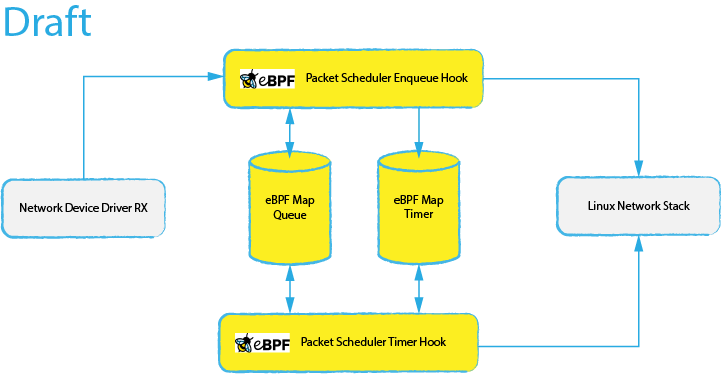
\includegraphics[width=\linewidth]{ebpf_pps_flow.png} %% This image is outdated and does not relfect the text.
  \label{fig:ebpf_pps_flow}
\end{figure}

Our vision is to create an eBPF based programmable packet scheduling framework
that is flexible enough to share between XDP and a Qdisc. We concluded that
there are four necessary components needed for such a framework, shown in figure
\ref{fig:ebpf_pps_flow}.

\begin{itemize}
        \item A PIFO/Eiffel eBPF map for queing packets.
        \item A enqueue eBPF hook responsible for redirecting packets to the PIFO/Eiffel eBPF map.
        \item A dequeue eBPF hook responsible for dequing the next packet from the PIFO/Eiffel eBPF map.
        \item Optionally, an eBPF based timer that handles pacing.
\end{itemize}

In our representation, we have decided that the best course of action was to
create a new eBPF map type for our Eiffel-based queue structures. Due to eBPF's
instruction count constraint, we would like to ensure that we are not wasting
instructions on queue manipulation by using a map type with helper functions.
Also, by using a new map type, we allow more flexibility by manipulating the
queues outside of the eBPF queuing hook.

From a programmer's perspective, the eBPF hook references the queues using
identifiers to the specific queues in the map. It is then up to the enqueue and
dequeue hooks to decide which queue to direct the packet using those identities.
The enqueue hook is different depending on if we are using XDP or a Qdisc. In
XDP, the enqueue hook is an XDP program that redirects the packet to an eBPF map
using XDP\_REDIRECT. Furthermore, the network device driver now provides a new
hook responsible for dequeuing packets from the queue maps. This hook returns a
reference to a dequeued packet. However, because the eBPF verifier does not
allow returning a direct pointer to the packet, the verifier is now aware of the
packets using BTF. The device driver supports bulking of packets by repeatedly
calling the dequeue hook before it does the transfer.

To introduce shaping into our new programmable scheduling framework, we use the
newly introduced eBPF timers API. The API implements timers using a new struct
type that we can store inside eBPF maps and supports both microsecond and
nanosecond precision, using the \textit{hrtimers} in the Linux kernel. In our
packet scheduling algorithms, these timers call eBPF hooks that manipulate the
Eiffel maps for the driver to dequeue later.


\section{eBPF-Qdisc}

\begin{itemize}
  \item Explain the building blocks of Cong Wang's eBPF-Qdisc.
  \item Explain that is a classfull Qdisc.
  \item Explain what changes are needed to make it better.
  \item Explain the limitations of the eBPF-Qdisc.
\end{itemize}


\section{eXpress Data Queueing (XDQ)}
% Frey: Should we just say ``XDP quing'' or ''Queing in XDP`` I personally don't like not having a name.

% Frey: Here, I would like to have an image that shows the design when we have created the complete picture.

Our design extends XDP by adding a new dequeue hook into the network drivers. We
rely on standard XDP to enqueue packets into BPF queue maps. However, the new
dequeue hook supports bulking by having the driver repeatedly dequeue packets
from the dequeue hook before it transmits the packets.


\section{Evaluation of eBPF-Qdisc and XDQ}

\begin{itemize}
  \item Compare a type of scheduling algorithm using eBPF-Qdisc and XDQ performance to Qdiscs that does the same functionality.
  \item Compare eBPF-Qdisc and XDQ performance to eachother.
\end{itemize}

\section{Conclusion}

\begin{itemize}
  \item Reiterate main points of design, and summarise results.
\end{itemize}



\bibliographystyle{ACM-Reference-Format}
\bibliography{references}


\end{document}
\endinput
